\chapter{Background}
\label{chapter: background}

\section{Edge Computing}
\label{sec: bg-edge}

\begin{figure*}[t]
\begin{minipage}[c]{2.5in}
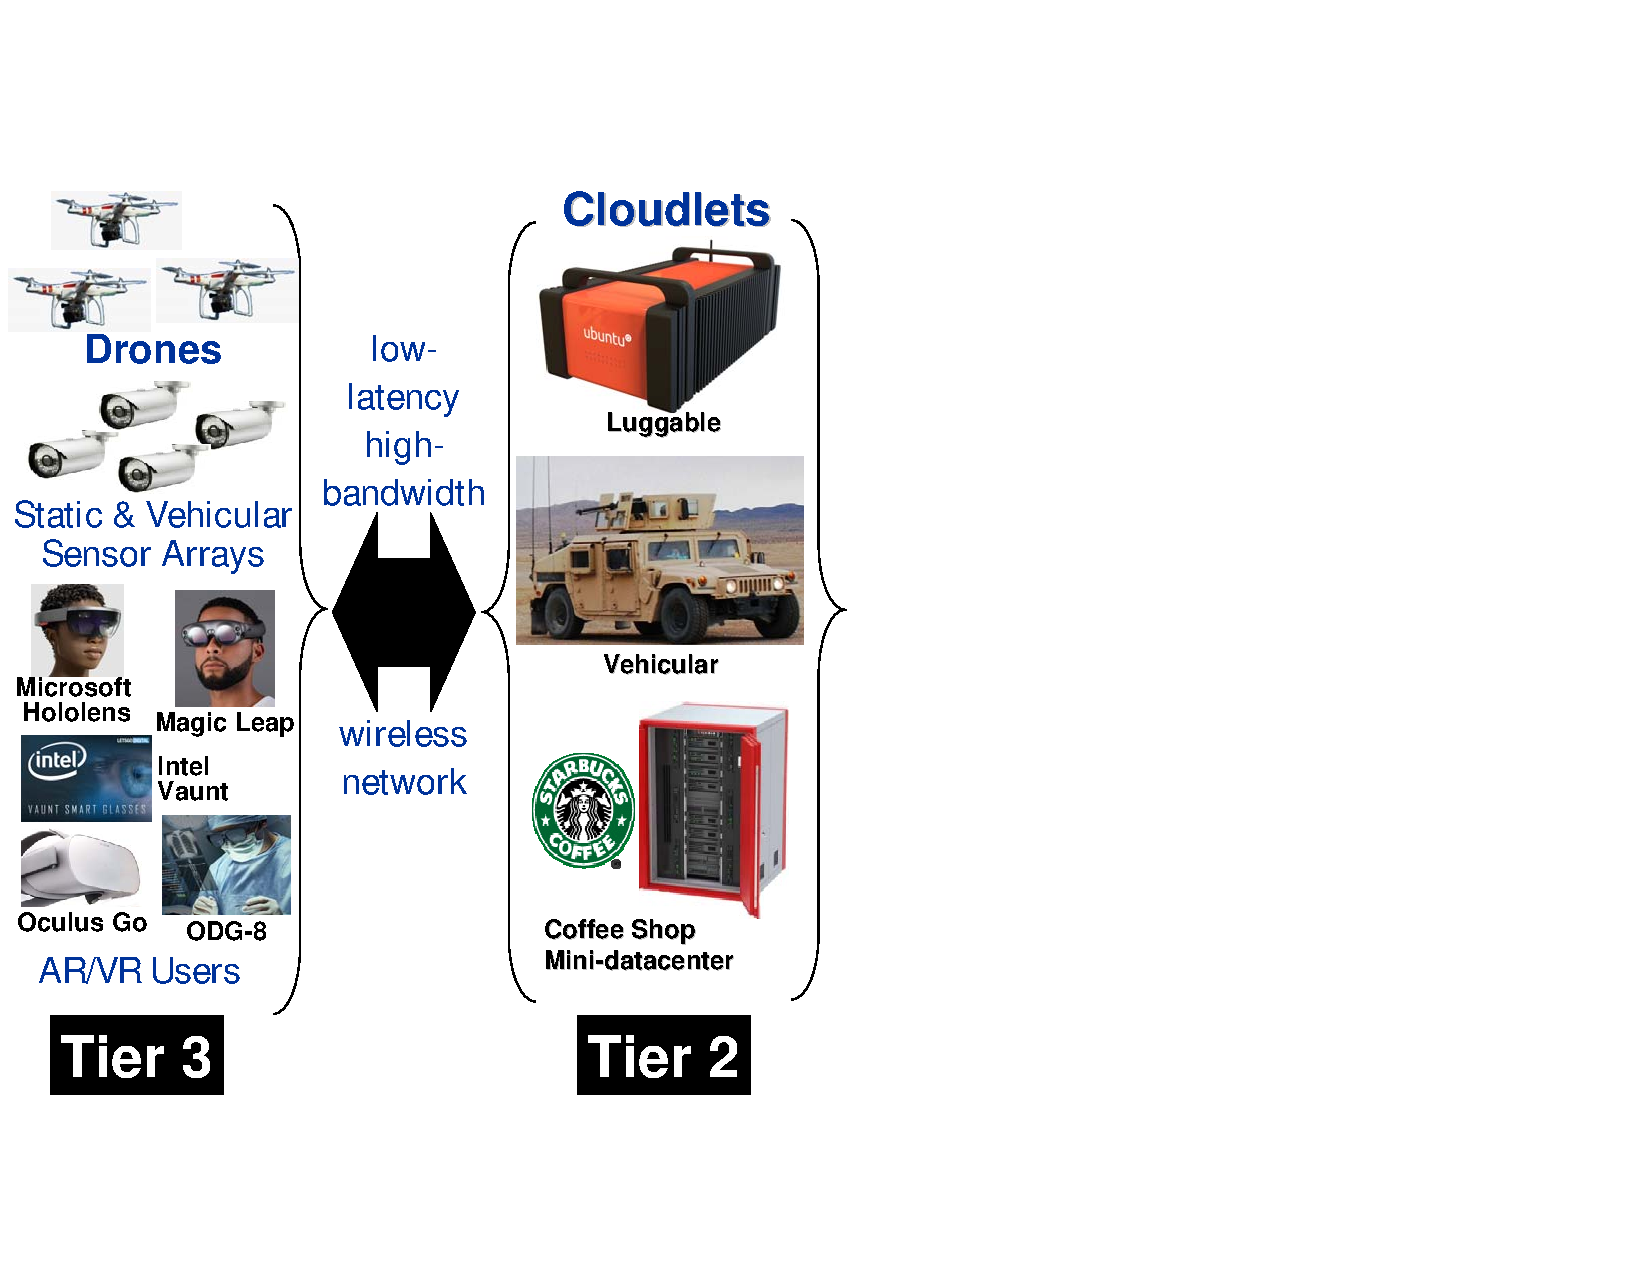
\includegraphics[scale=0.45]{FIGS/fig-3tier-A.pdf}
\end{minipage}
\begin{minipage}[c]{2.7in}
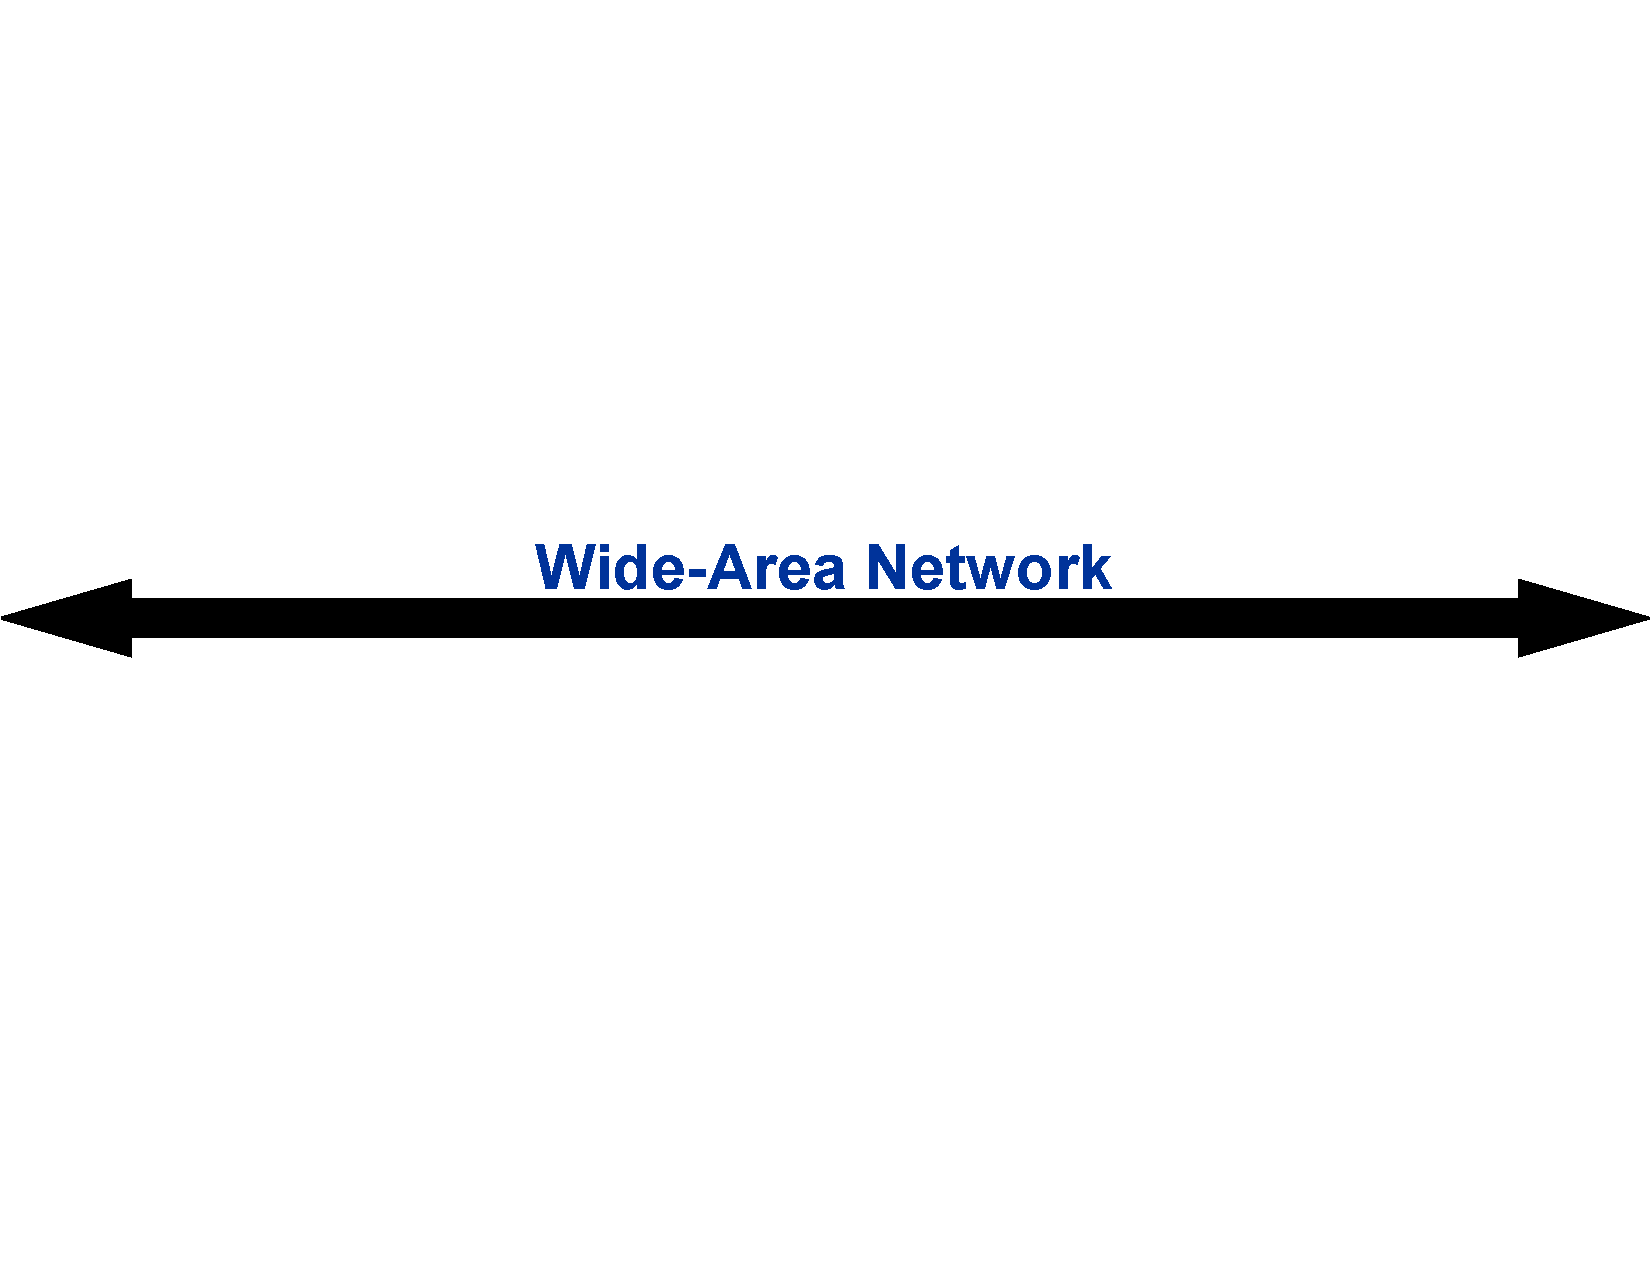
\includegraphics[scale=0.25]{FIGS/fig-3tier-B-cropped.pdf}\\
\end{minipage}
\begin{minipage}[c]{1in}
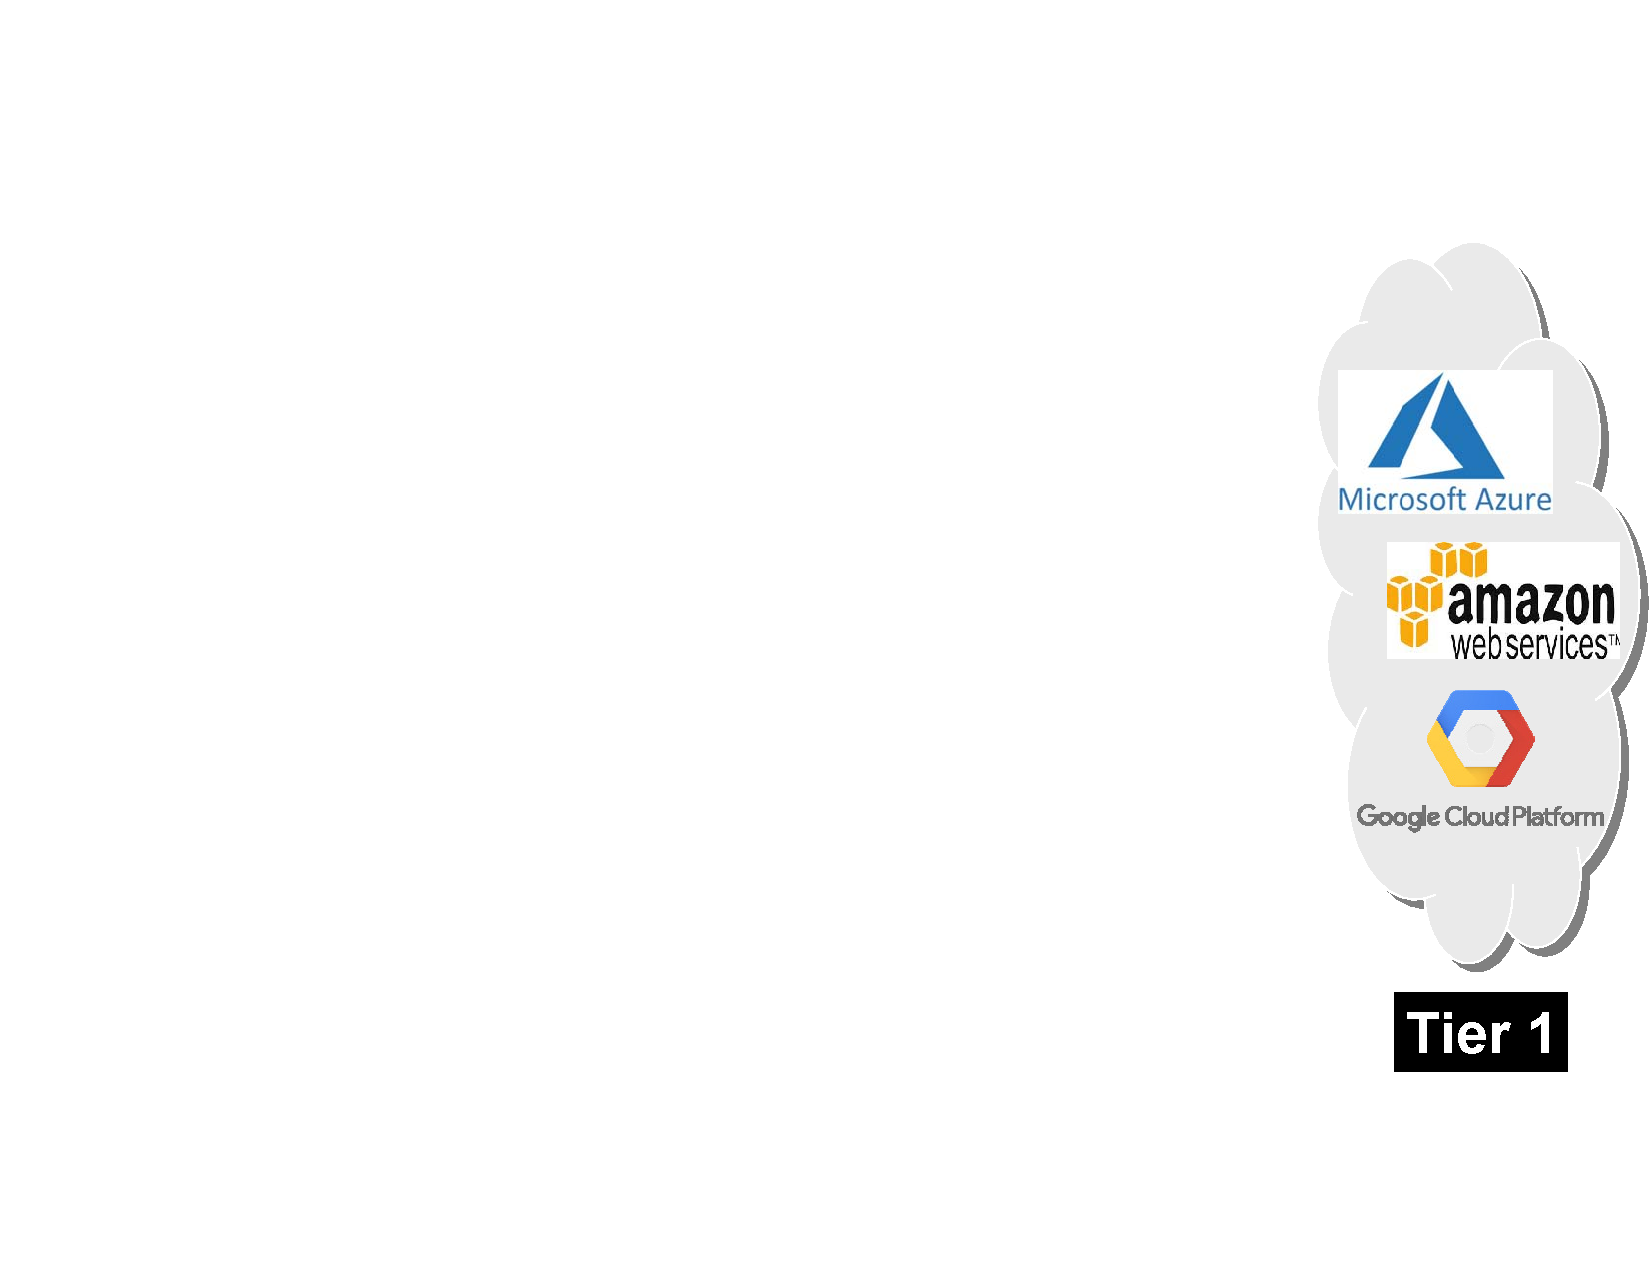
\includegraphics[scale=0.45]{FIGS/fig-3tier-C.pdf}
\end{minipage}
\caption{\small Tiered Model of Computing}
\label{fig:3tier}
\end{figure*}

{\em Edge computing} is a nascent computing paradigm that has gained
considerable traction over the past few years. It champions the idea of placing
substantial compute and storage resources at the edge of the Internet, in close
proximity to mobile devices or sensors.  Terms such as
``cloudlets''~\cite{Satya2009}, ``micro data centers (MDCs)''~\cite{Greene2012},
``fog''~\cite{Bonomi2012}, and ``mobile edge computing (MEC)''~\cite{Brown2013}
are used to refer to these small, edge-located computing nodes.  We use these
terms interchangably in the rest of this thesis. Edge computing is motivated by
its potential to improve latency, bandwidth, and scalability over a cloud-only
model.  More practically, some efforts stem from the drive towards
software-defined networking (SDN) and network function virtualization (NFV), and
the fact that the same hardware can provide SDN, NFV, and edge computing
services. This suggests that infrastructure providing edge computing services
may soon become ubiquitous, and may be deployed at greater densities than
content delivery network (CDN) nodes today. 

Satya et al.~\cite{satya2019computing} best describes the modern computing
landscape with edge computing using a tiered model, shown in
Figure~\ref{fig:3tier}. Tiers are separated by distinct yet stable sets of
design constraints. From left to right, this tiered model represents a hierarchy
of increasing physical size, compute power, energy usage, and elasticity. Tier-1
represents today's large-scale and heavily consolidated data-centers. Compute
elasticity and storage permanence are two dominating themes here. Tier-3
represents IoT and mobile devices, which are constrained by their physical size,
weight, and heat dissipation. Sensing is the key functionality of tier-3
devices. For example, today's smartphones are already rich in sensors, including
camera, microphone, accelerometers, gyroscopes and GPS. In addition, an
increasing amount of IoT devices with specific sensing modalities are getting
adopted, e.g. smart speakers, security cameras, and smart thermostats. 

With the large-scale deployment of tier-3 devices, there exists a tension
between the gigantic amount of data collected and generated by them and their
limited capabilities to process these data on-board. For example, most
surveillance cameras are limited in computation to run state-of-art computer
vision algorithms to analyze the videos they capture. To overcome this tension,
a tier-3 device could offload computation over network to tier-1. This
capability was first demonstrated in 1997 by Noble et al.~\cite{Noble1997}, who
used it to implement speech recognition with acceptable performance on a
resource-limited mobile device. In 1999, Flinn et al.~\cite{Flinn1999} extended
this approach to improve battery life.  These concepts were generalized in a
2001 paper that introduced the term {\em cyber foraging} for the amplification
of a mobile device's data or compute capabilities by leveraging nearby
infrastructure~\cite{Satya2001}.  Thanks to these research efforts, computation
offloading is widely used by IoT devices today. For example, when a user asks an
Amazon Echo smart speaker ``Alexa, what is the weather today?'', the user's
audio stream is captured by the smart speaker and transmitted to the cloud for
speech recognition, text understanding, and question answering.

However, offloading computation to the cloud has its own downside. Because of
the consolidation needed to achieve the economy of scale, today's datacenters
are ``far'' from tier-3 devices. The latency, throughput, and cost of wide-area
network (WAN) significantly limit the amount of applications that can benefit
from computation offloading. Even worse, it is the logical distance in the
network that matters rather than the physical distance. Routing decisions in
today's Internet are made locally and are based on business agreements,
resulting in suboptimal solutions. For example, using traceroute, we determine
that a LTE packet originating from a smartphone on the campus of Carnegie Mellon
University (CMU) in Pittsburgh to a nearby server actually traverses to
Philedelphia, a city several hundreds miles away. This is because Philidephia
has the nearest peering point of the particular commercial LTE network in use to
the public Internet. In 2010, Li et al.~\cite{li2010cloudcmp} report that the
average round trip time (RTT) from 260 global vantage points to their optimal
Amazon EC2 instances is 74 ms. In addition to long network delay, the high
network fan-in of datacenters means its aggregation network need to carry
significant amount of traffic. As the number of tier-3 devices is expected to
grow exponentially, these network links face significant challenges to handle
the ever-increasing volume of ingress traffic. 

\begin{figure}
\begin{minipage}[c]{3in}
\begin{center}
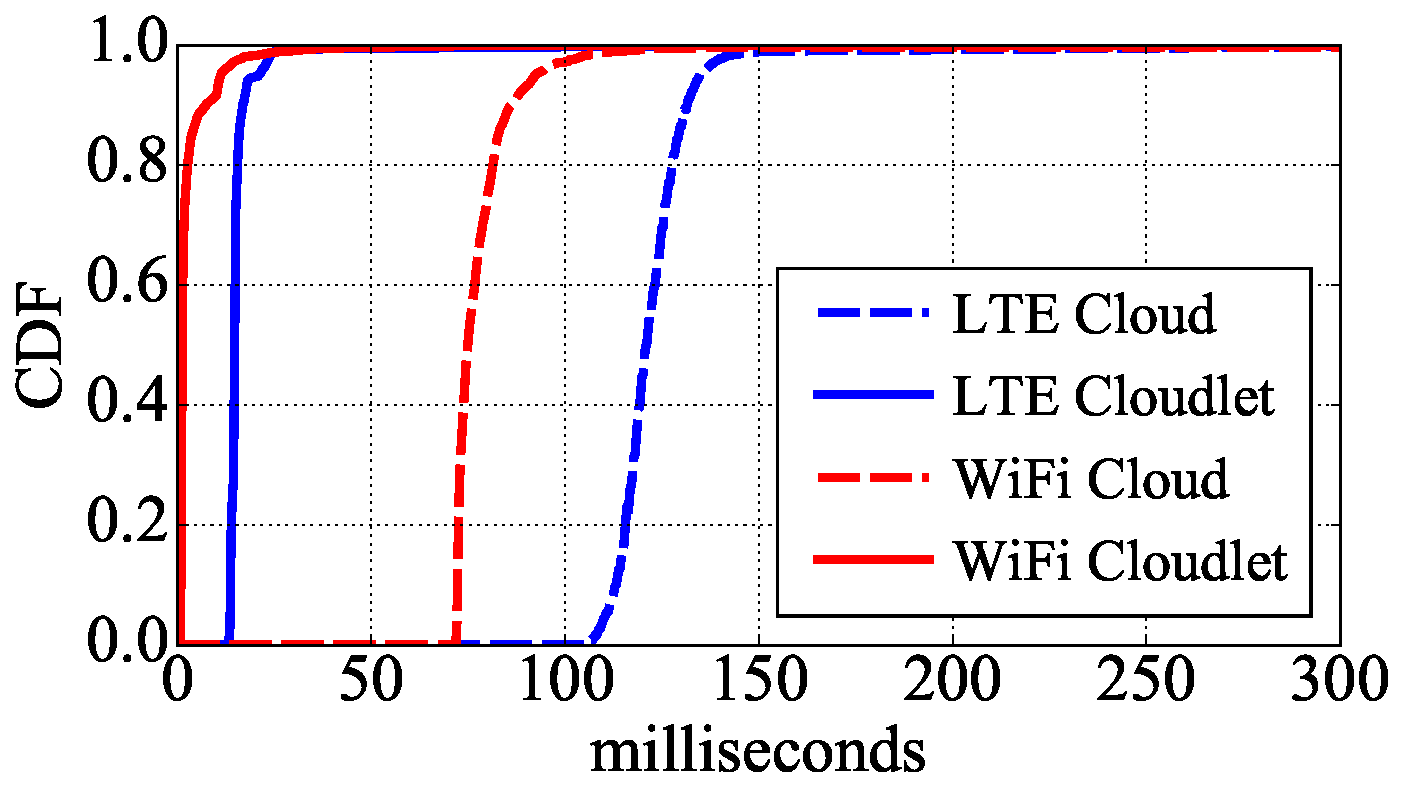
\includegraphics[height=1.5in]{FIGS/ping_cdf.pdf}
\caption{CDF of pinging RTTs}
\label{fig:ping-CDF}
\end{center}
\end{minipage}
\begin{minipage}[c]{3.5in}
\begin{center}
    \hspace{0.2in}
    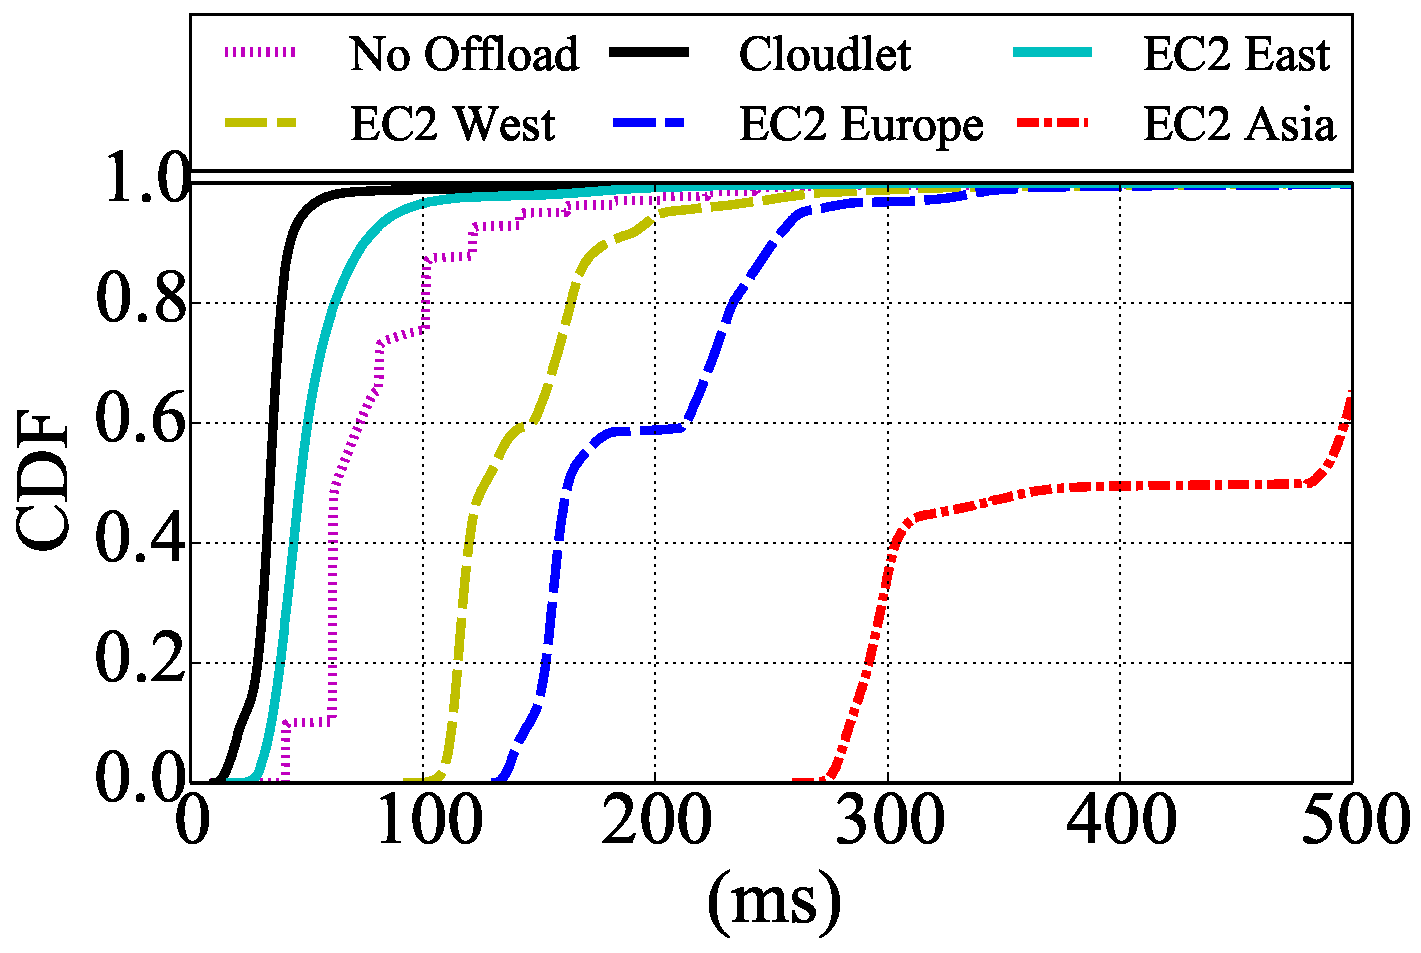
\includegraphics[width=0.8\textwidth,clip,trim=91pt 376pt 0 0]{FIGS/Legend-Wifi.pdf}
    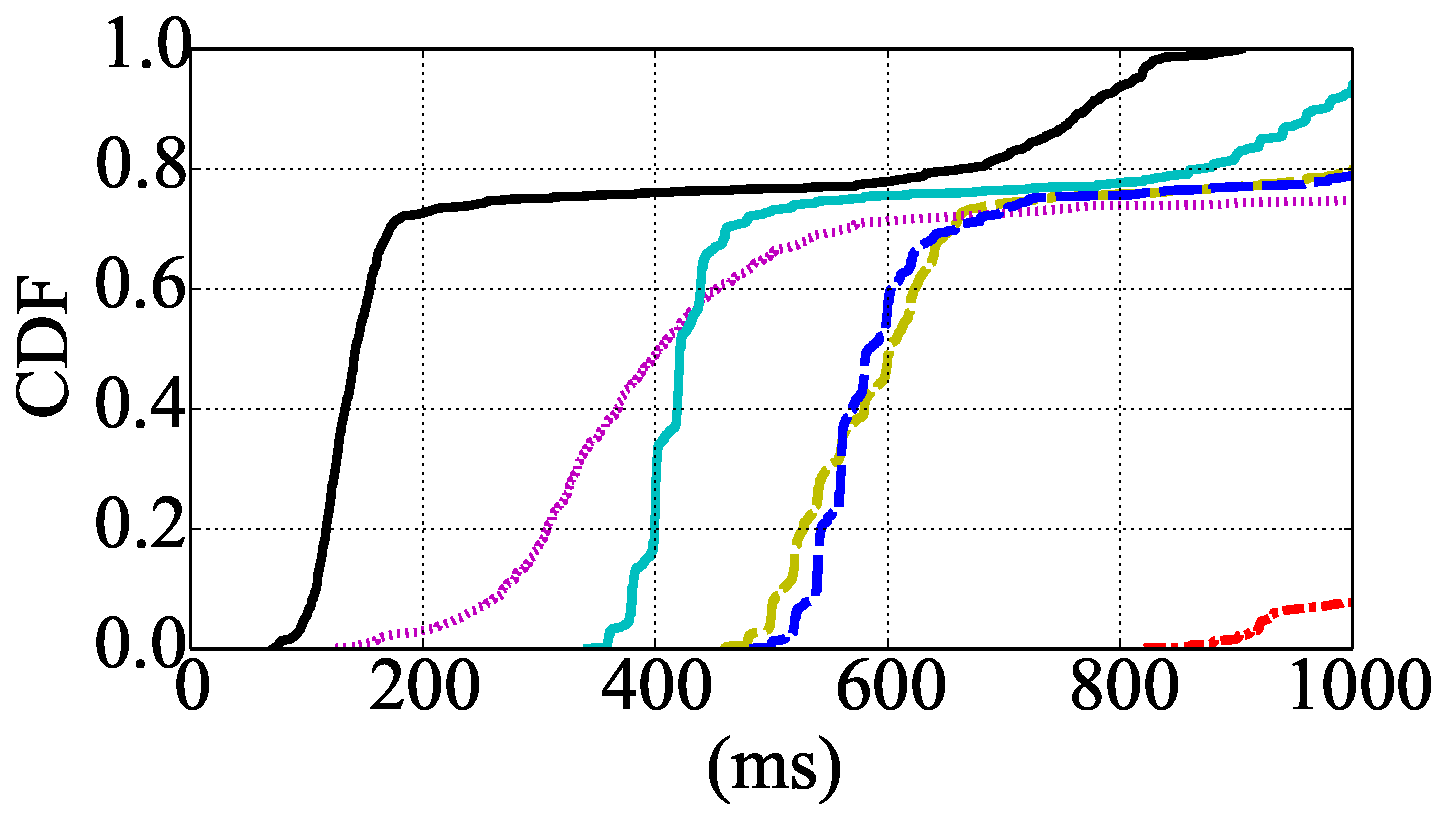
\includegraphics[width=3in]{FIGS/Face-LTE.pdf}
\caption{FACE Response Time over LTE}
\label{fig:response-time-lte-face}
\end{center}
\end{minipage}
\end{figure}

To counter these problems, edge computing, shown as the tier-2 in
Figure~\ref{fig:3tier}, is proposed. Cloudlets at tier-2 creates the illusion of
bringing Tier-1 ``closer''. They are featured by their network proximity to
tier-3 devices and their significantly larger compute and storage compared to
tier-3 devices. While tier-3 devices typically run on battery and are optimized
for low energy consumption, saving energy is not a major concern for tier-2 as
they are either plugged into the electric grid or powered by other sources of
energy (e.g. fuels in a vehicle). Cloudlets serve two purposes in the tiered
model. First, they provide infrastructure for compute-intensive and
latency-sensitive applications for tier-3. Wearable cognitive assistance is an
examplar of these applications. Second, by processing data closer to the source
of the content, it reduces the excessive traffic going into tier-1 datacenters.
Figure~\ref{fig:ping-CDF} shows the RTT comparison of PING to the cloud and the
cloudlet over WiFi and LTE. Cloudlet's RTT is on average 80 to 100ms shorter
than its counterpart to the cloud. Figure~\ref{fig:response-time-lte-face} shows
the impact of network latency on an application that recognizes faces. Three
offloading scenarios are considered: offloading to the cloud, offloading to the
cloudlet, and no offloading. The data transmitted are images captured by a
smartphone. As we can see, the limited bandwidth of the cellular network further
worsen the response time when offloading to the cloud. In fact, for this
particular application, even local execution outperforms offloading to the
nearest cloud due to network delay. The optimal computational offload location
is cloudlet, whose median response time is more than 200ms faster than local
execution and about 250 ms faster than the nearest cloud.

The low-latency and high-bandwidth compute infrastructure provided by cloudlets
is an indispensible foundation for latency-sensitive and compute-intensive
wearable cognitive assistance. Cloudlet also poses unique challenges for
scalability as resources are a lot more limited compared to datacenters. How to
scale WCAs to many users using cloudlets is the key question this thesis set out to
investigate. 


\section{Gabriel Platform}
\label{sec: bg-gabriel}

\begin{figure}
\centering
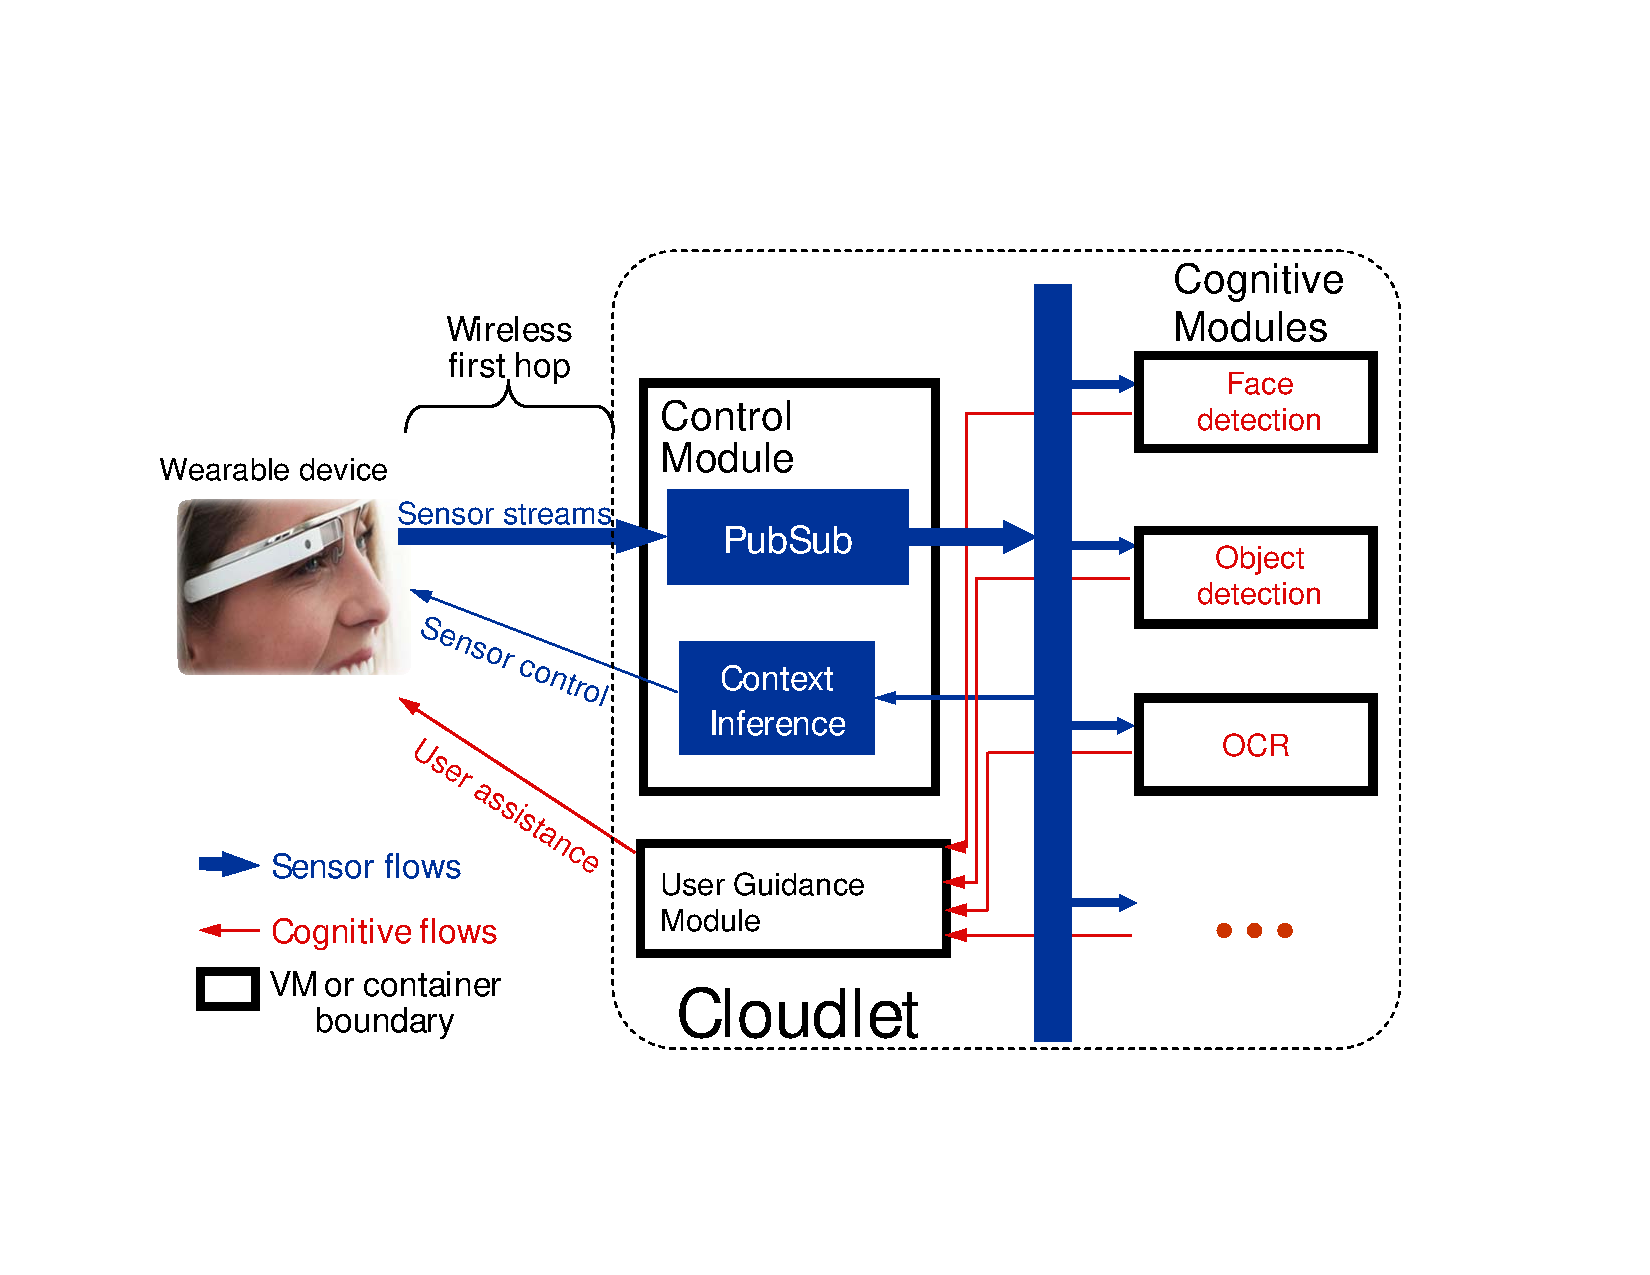
\includegraphics[width=0.8\linewidth]{FIGS/fig-backend-structure-simple-crop.pdf}
\begin{captiontext}
{\rm (Source: Chen et al~\cite{chen2017empirical})}
\end{captiontext}
\caption{\small Gabriel Platform}
\label{fig:gabriel}
\end{figure}

The Gabriel platform~\cite{ha2014towards,chen2017empirical}, shown in
Figure~\ref{fig:gabriel}, is an application framework for wearable cognitive
assistance. It consists of a front-end running on wearable devices and a
back-end running on cloudlets. The Gabriel front-end performs preprocessing of
sensor data (e.g., compression and encoding), which it then streams over a
wireless network to a cloudlet.  The Gabriel back-end on the cloudlet has a
modular structure. The {\em control module} is the focal point for all
interactions with the wearable device.  A publish-subscribe (PubSub) mechanism
decodes and distributes the incoming sensor streams to multiple {\em cognitive
modules} (e.g., task-specific computer vision algorithms) for concurrent
processing. Cognitive module outputs are integrated by a task-specific {\em user
guidance module} that performs higher-level cognitive processing such as
inferring task state, detecting errors, and generating guidance in one or more
modalities (e.g., audio, video, text, etc.).

The original Gabriel platform was built with a single user in mind,
and did not have mechanisms to share cloudlet resources in a
controlled manner.  It did, however, have a token-based transmission
mechanism.  This limited a client to only a small number of
outstanding operations, thereby offering a simple form of rate
adaptation to processing or network bottlenecks.  We have retained
this token mechanism in our system, described in the rest of this paper.
In addition, we have extended Gabriel with new mechanisms to handle
multitenancy, perform resource allocation, and support
application-aware adaptation.  We refer to the two versions of the
platform as ``Original Gabriel'' and ``Scalable Gabriel.''

\section{Example Gabriel Applications}

Many applications have been built on top of the Gabriel platform.  Recent
papers~\cite{chen2017empirical}~\cite{chen2018application} describe these applications,
along with detailed analysis of their end-to-end latency. For example, the LEGO
application guides a user to construct a Lego model, step by step, continuously
monitoring the task with computer vision, and providing instructions when it has
detected that the user has completed a step. POOL assists a user in aiming a
pool cue stick. PING PONG suggests hitting a ball to the left or right to win a
rally in table tennis. FACE recognizes a face that has appeared in a scene,
searches the user's personal database, and whispers the person's name. IKEA
helps a user to assemble an IKEA lamp step by step.

These applications run on multiple wearable devices such as Google
Glass, Microsoft HoloLens, Vuzix Glass, and ODG R7. At a high level, 
the cloudlet workflows of these applications are similar, and consist of
two major phases.  The first phase uses computer vision
to extract a symbolic, idealized representation of the state of the
task, accounting for real-world variations in lighting, viewpoint,
etc.  The second phase operates on the symbolic representation,
implements the logic of the task at hand, and occasionally generates
guidance for the user.  In most WCA applications, the first phase is
far more compute intensive than the second phase.

